% Lifting Autogyro Unit --- Cross-Section v4
% Wider layout, spread labels, clean hub area
% Compile: pdflatex assembly_v4.tex
\documentclass{article}
\usepackage[paperwidth=38cm,paperheight=30cm,margin=0.3cm]{geometry}
\usepackage{amsmath,amssymb,tikz}
\usetikzlibrary{arrows.meta,calc,patterns,decorations.pathreplacing,positioning}
\pagestyle{empty}

\begin{document}
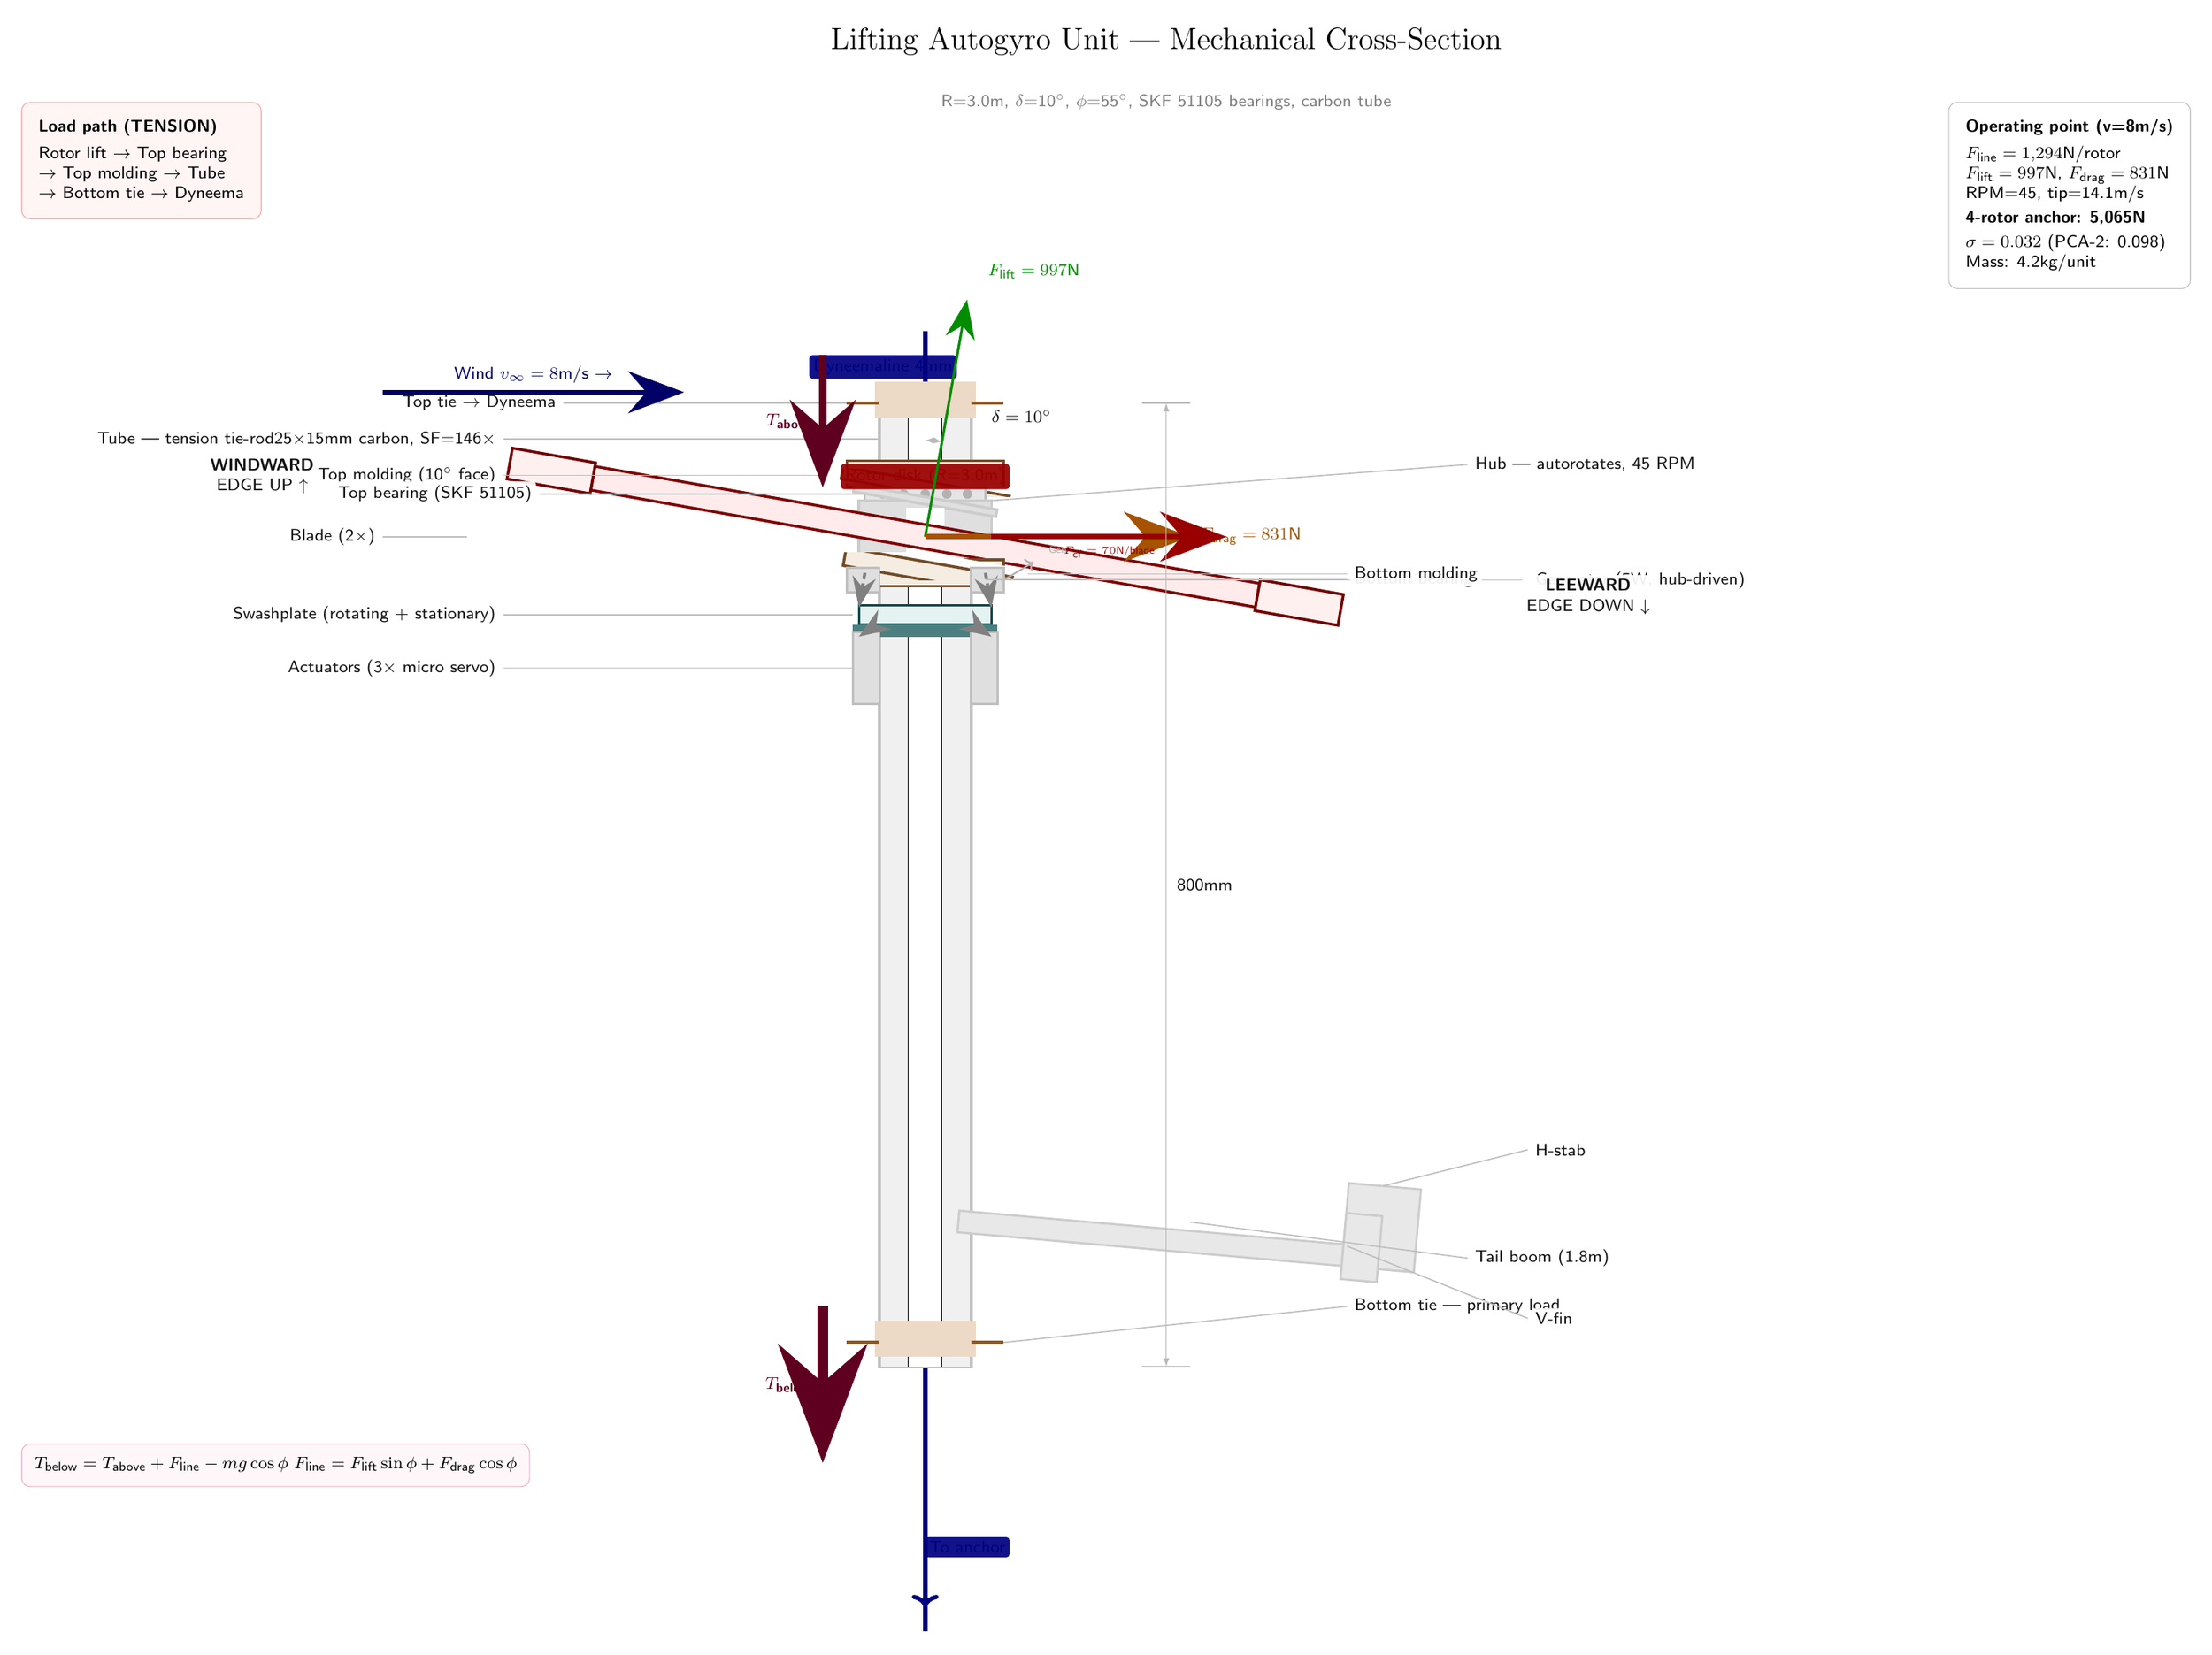
\begin{tikzpicture}[
    scale=2.0,
    dyneema/.style={draw=blue!50!black, line width=2.0pt},
    tube/.style={draw=gray!50, fill=gray!12, line width=1.5pt},
    molding/.style={draw=brown!60!black, fill=brown!15, line width=1.3pt},
    bearing/.style={draw=gray!50, fill=gray!20, line width=1.0pt},
    hub/.style={draw=gray!40, fill=gray!25, line width=1.3pt},
    rotor/.style={draw=red!50!black, fill=red!8, line width=1.3pt},
    blade/.style={draw=red!45!black, fill=red!6, line width=1.3pt},
    actuator/.style={draw=gray!50, fill=gray!25, line width=1.0pt},
    swash/.style={draw=teal!60!black, fill=teal!10, line width=1.0pt},
    empennage/.style={draw=gray!40, fill=gray!18, line width=1.0pt},
    generator/.style={draw=gray!50, fill=gray!25, line width=1.0pt},
    force/.style={-{Stealth[scale=2.2]}, line width=2.5pt},
    forcecomp/.style={-{Stealth[scale=1.5]}, line width=1.5pt, densely dashed},
    dimline/.style={latex-latex, thin, draw=gray!55},
    dimext/.style={thin, draw=gray!55},
    % Leader line for labels
    lead/.style={line width=0.6pt, gray!50},
    annot/.style={font=\footnotesize\sffamily, fill=white, fill opacity=0.93, inner sep=2pt, rounded corners=1.5pt},
    label/.style={font=\small\sffamily\bfseries},
]

\def\tilt{10}
\def\tubetop{8.0}\def\tubebot{0}
\def\toptieZ{8.0}
\def\topmoldZ{7.3}\def\topbearZ{7.3}
\def\hubtopZ{7.19}\def\rotorZ{6.89}\def\hubbotZ{6.59}
\def\botbearZ{6.59}\def\botmoldZ{6.48}
\def\genZ{6.53}\def\swashZ{6.1}\def\actZ{5.5}
\def\empZ{1.2}\def\bottieZ{0.2}
\def\moldH{0.22}\def\bearingH{0.11}\def\hubH{0.6}

% ============================================================
% CENTERLINE ASSEMBLY
% ============================================================

% Dyneema
\draw[dyneema] (0, \tubebot-2.2) -- (0, \tubetop+0.6);
\node[annot, blue!50!black] at (-0.35, \tubetop+0.3) {Dyneema\\line 4mm};

% Tube
\fill[tube] (-0.38, \tubebot) rectangle (0.38, \tubetop);
\draw[tube] (-0.38, \tubebot) -- (-0.38, \tubetop) -- (0.38, \tubetop) -- (0.38, \tubebot);
\fill[white] (-0.14, \tubebot) rectangle (0.14, \tubetop);
\draw[thin] (-0.14, \tubebot) -- (-0.14, \tubetop);
\draw[thin] (0.14, \tubebot) -- (0.14, \tubetop);

% Top tie
\fill[brown!30] (-0.42, \toptieZ-0.12) rectangle (0.42, \toptieZ+0.18);
\draw[brown!70!black, line width=1.5pt] (-0.65, \toptieZ) -- (-0.38, \toptieZ);
\draw[brown!70!black, line width=1.5pt] (0.38, \toptieZ) -- (0.65, \toptieZ);

% Top molding
\fill[molding] (-0.65, \topmoldZ) rectangle (0.65, \topmoldZ+\moldH);
\begin{scope}
    \clip (-1.0, \topmoldZ-0.08) rectangle (1.0, \topmoldZ+0.15);
    \fill[white, rotate around={-\tilt:(0,\topmoldZ)}] (-1.0, \topmoldZ-0.08) rectangle (1.0, \topmoldZ+0.12);
    \fill[molding, rotate around={-\tilt:(0,\topmoldZ)}] (-0.7, \topmoldZ-0.05) rectangle (0.7, \topmoldZ+0.05);
\end{scope}

% Top bearing
\fill[bearing] (-0.5, \topbearZ-\bearingH) rectangle (0.5, \topbearZ);
\foreach \x in {-0.35,-0.18,0,0.18,0.35} { \fill[gray!60] (\x, \topbearZ-\bearingH/2) circle (0.04); }

% Hub
\fill[hub] (-0.55, \hubbotZ) rectangle (0.55, \hubtopZ);
\fill[hub, rotate around={-\tilt:(0,\hubtopZ)}] (-0.6, \hubtopZ-0.03) rectangle (0.6, \hubtopZ+0.03);
\fill[hub, rotate around={-\tilt:(0,\hubbotZ)}] (-0.6, \hubbotZ-0.03) rectangle (0.6, \hubbotZ+0.03);
\fill[white] (-0.16, \hubbotZ+0.06) rectangle (0.16, \hubtopZ-0.06);

% Rotor disk + blades
\begin{scope}[rotate around={-\tilt:(0,\rotorZ)}]
    \fill[rotor] (-2.8, \rotorZ-0.1) rectangle (2.8, \rotorZ+0.1);
    \fill[blade] (-3.5, \rotorZ-0.13) rectangle (-2.8, \rotorZ+0.13);
    \fill[blade] (2.8, \rotorZ-0.13) rectangle (3.5, \rotorZ+0.13);
\end{scope}

% Bottom bearing
\fill[bearing] (-0.5, \botbearZ-\bearingH) rectangle (0.5, \botbearZ);
\foreach \x in {-0.35,-0.18,0,0.18,0.35} { \fill[gray!60] (\x, \botbearZ-\bearingH/2) circle (0.04); }

% Bottom molding
\fill[molding] (-0.65, \botmoldZ) rectangle (0.65, \botmoldZ+\moldH);
\begin{scope}
    \clip (-1.0, \botmoldZ+0.05) rectangle (1.0, \botmoldZ+0.28);
    \fill[white, rotate around={-\tilt:(0,\botmoldZ)}] (-1.0, \botmoldZ+0.12) rectangle (1.0, \botmoldZ+0.28);
    \fill[molding, rotate around={-\tilt:(0,\botmoldZ)}] (-0.7, \botmoldZ+0.05) rectangle (0.7, \botmoldZ+0.2);
\end{scope}

% Generator
\fill[generator] (0.38, \genZ-0.1) rectangle (0.65, \genZ+0.1);
\fill[generator] (-0.38, \genZ-0.1) rectangle (-0.65, \genZ+0.1);

% Swashplate
\fill[swash] (-0.55, \swashZ+0.06) rectangle (0.55, \swashZ+0.22);
\fill[teal!40!gray] (-0.6, \swashZ-0.04) rectangle (0.6, \swashZ+0.06);
\draw[forcecomp, gray] (0.5, \hubbotZ) -- (0.55, \swashZ+0.2);
\draw[forcecomp, gray] (-0.5, \hubbotZ) -- (-0.55, \swashZ+0.2);

% Actuators
\fill[actuator] (0.38, \actZ) rectangle (0.6, \actZ+0.6);
\fill[actuator] (-0.38, \actZ) rectangle (-0.6, \actZ+0.6);
\draw[forcecomp, gray] (0.49, \actZ+0.6) -- (0.55, \swashZ-0.04);
\draw[forcecomp, gray] (-0.49, \actZ+0.6) -- (-0.55, \swashZ-0.04);

% Empennage
\begin{scope}[shift={(0.38, \empZ)}, rotate around={-5:(0,\empZ)}]
    \fill[empennage] (0, -0.09) rectangle (3.8, 0.09);
    \fill[empennage] (3.2, -0.09) rectangle (3.8, 0.6);
    \fill[empennage] (3.2, 0.35) rectangle (3.5, -0.2);
\end{scope}

% Bottom tie
\fill[brown!30] (-0.42, \bottieZ-0.12) rectangle (0.42, \bottieZ+0.18);
\draw[brown!70!black, line width=1.5pt] (-0.65, \bottieZ) -- (-0.38, \bottieZ);
\draw[brown!70!black, line width=1.5pt] (0.38, \bottieZ) -- (0.65, \bottieZ);

% Generator callout
\draw[->, gray!60, line width=0.8pt] (0.65, \genZ) -- (0.9, \genZ+0.15);
\node[font=\tiny\sffamily, gray!60] at (1.1, \genZ+0.25) {Gen};

% Anchor extension
\draw[dyneema, ->] (0, \tubebot-1.0) -- (0, \tubebot-2.0);
\node[annot, blue!50!black] at (0.35, \tubebot-1.5) {To anchor};

% ============================================================
% LABELS --- staggered LEFT and RIGHT, long leader lines
% ============================================================

% LEFT side labels
\draw[lead] (-0.38, \tubetop-0.3) -- (-3.5, \tubetop-0.3);
\node[annot, left=0.05cm] at (-3.5, \tubetop-0.3) {Tube --- tension tie-rod\\25$\times$15mm carbon, SF=146$\times$};

\draw[lead] (-0.65, \toptieZ) -- (-3.0, \toptieZ);
\node[annot, left=0.05cm] at (-3.0, \toptieZ) {Top tie $\rightarrow$ Dyneema};

\draw[lead] (-0.85, \topmoldZ+0.1) -- (-3.5, \topmoldZ+0.1);
\node[annot, left=0.05cm] at (-3.5, \topmoldZ+0.1) {Top molding (10$^\circ$ face)};

\draw[lead] (-0.5, \topbearZ-\bearingH/2) -- (-3.2, \topbearZ-\bearingH/2);
\node[annot, left=0.05cm] at (-3.2, \topbearZ-\bearingH/2) {Top bearing (SKF 51105)};

\draw[lead] (-0.6, \swashZ+0.14) -- (-3.5, \swashZ+0.14);
\node[annot, left=0.05cm] at (-3.5, \swashZ+0.14) {Swashplate (rotating + stationary)};

\draw[lead] (-0.6, \actZ+0.3) -- (-3.5, \actZ+0.3);
\node[annot, left=0.05cm] at (-3.5, \actZ+0.3) {Actuators (3$\times$ micro servo)};

% RIGHT side labels — staggered vertically to avoid overlap
\draw[lead] (0.55, \hubtopZ) -- (4.5, \hubtopZ+0.3);
\node[annot, right=0.05cm] at (4.5, \hubtopZ+0.3) {Hub — autorotates, 45 RPM};

\draw[lead] (0.65, \genZ) -- (5.0, \genZ);
\node[annot, right=0.05cm] at (5.0, \genZ) {Generator (5W, hub-driven)};

\draw[lead] (0.5, \botbearZ-\bearingH/2) -- (3.5, \botbearZ-\bearingH/2);
\node[annot, right=0.05cm] at (3.5, \botbearZ-\bearingH/2) {Bottom bearing};

\draw[lead] (0.85, \botmoldZ+0.1) -- (3.5, \botmoldZ+0.1);
\node[annot, right=0.05cm] at (3.5, \botmoldZ+0.1) {Bottom molding};

\draw[lead] (0.65, \bottieZ) -- (3.5, \bottieZ+0.3);
\node[annot, right=0.05cm] at (3.5, \bottieZ+0.3) {Bottom tie — primary load};

% Blade label (left of disk)
\draw[lead] (-3.8, \rotorZ) -- (-4.5, \rotorZ);
\node[annot, left=0.05cm] at (-4.5, \rotorZ) {Blade (2$\times$)};

% Empennage labels
\draw[lead] (2.2, \empZ+0.0) -- (4.5, \empZ-0.3);
\node[annot, right=0.05cm] at (4.5, \empZ-0.3) {Tail boom (1.8m)};
\draw[lead] (3.8, \empZ+0.3) -- (5.0, \empZ+0.6);
\node[annot, right=0.05cm] at (5.0, \empZ+0.6) {H-stab};
\draw[lead] (3.5, \empZ-0.2) -- (5.0, \empZ-0.8);
\node[annot, right=0.05cm] at (5.0, \empZ-0.8) {V-fin};

% ============================================================
% DISK EDGE LABELS + TILT
% ============================================================
% Edge labels — further out, clear of blades
\node[annot, align=center] at (-5.5, \rotorZ+0.5) {\bfseries WINDWARD\\\footnotesize EDGE UP $\uparrow$};
\node[annot, align=center] at (5.5, \rotorZ-0.5) {\bfseries LEEWARD\\\footnotesize EDGE DOWN $\downarrow$};
\node[annot, red!60!black] at (0, \rotorZ+0.5) {Rotor disk (R=3.0m)};
\draw[dimline] (0, \rotorZ+0.8) arc[start angle=90, end angle={90-\tilt}, radius=0.8cm];
\node[annot] at (0.8, \rotorZ+1.0) {$\delta=10^\circ$};

% ============================================================
% FORCE ARROWS
% ============================================================
\draw[force, green!55!black, very thick] (0, \rotorZ) -- ++({2.0*sin(\tilt)}, {2.0*cos(\tilt)})
    node[above right=0.3cm, font=\footnotesize\sffamily, green!55!black] {$F_\text{lift}=997$N};

\draw[force, orange!65!black] (0, \rotorZ) -- ++(2.2, 0)
    node[right, font=\footnotesize\sffamily, orange!65!black] {$F_\text{drag}=831$N};

\draw[force, purple!50!black, line width=3.5pt] (-0.85, \tubetop+0.4) -- (-0.85, \topmoldZ)
    node[midway, left, font=\footnotesize\sffamily\bfseries, purple!50!black] {$T_\text{above}$};

\draw[force, purple!50!black, line width=5pt] (-0.85, \tubebot+0.5) -- (-0.85, \tubebot-0.8)
    node[midway, left, font=\footnotesize\sffamily\bfseries, purple!50!black] {$T_\text{below}$};

\draw[force, red!60!black, line width=2.5pt] (0.55, \rotorZ) -- (2.5, \rotorZ)
    node[midway, below, font=\tiny\sffamily, red!60!black] {$F_\text{cf}=70$N/blade};

% Wind
\draw[force, blue!40!black, line width=2.0pt] (-4.5, \rotorZ+1.2) -- (-2.0, \rotorZ+1.2)
    node[midway, above, font=\footnotesize\sffamily, blue!40!black] {Wind $v_\infty=8$m/s $\to$};

% ============================================================
% DIMENSIONS
% ============================================================
\draw[dimext] (1.8, \tubebot) -- (2.2, \tubebot);
\draw[dimext] (1.8, \tubetop) -- (2.2, \tubetop);
\draw[dimline] (2.0, \tubebot) -- (2.0, \tubetop);
\node[annot, right=0.1cm] at (2.0, 4.0) {800mm};

% ============================================================
% INFO PANELS --- outside drawing area
% ============================================================

% Load path --- far left
\node[draw=red!35, fill=red!4, rounded corners=4pt, inner sep=8pt,
      anchor=north west, font=\footnotesize\sffamily, align=left]
    at (-7.5, 10.5) {
    \textbf{Load path (TENSION)}\\[3pt]
    Rotor lift $\to$ Top bearing\\
    $\to$ Top molding $\to$ Tube\\
    $\to$ Bottom tie $\to$ Dyneema
};

% Operating point --- far right
\node[draw=black!25, fill=white, rounded corners=4pt, inner sep=8pt,
      anchor=north east, font=\footnotesize\sffamily, align=left]
    at (10.5, 10.5) {
    \textbf{Operating point (v=8m/s)}\\[3pt]
    $F_\text{line}=1,\!294$N/rotor\\
    $F_\text{lift}=997$N, $F_\text{drag}=831$N\\
    RPM=45, tip=14.1m/s\\[2pt]
    \textbf{4-rotor anchor: 5,065N}\\[2pt]
    $\sigma=0.032$ (PCA-2: 0.098)\\
    Mass: 4.2kg/unit
};

% Tension formula --- far left bottom
\node[draw=purple!30, fill=purple!3, rounded corners=4pt, inner sep=6pt,
      anchor=south west, font=\footnotesize\sffamily]
    at (-7.5, -1.0) {
    $T_\text{below}=T_\text{above}+F_\text{line}-mg\cos\phi$\\[2pt]
    $F_\text{line}=F_\text{lift}\sin\phi+F_\text{drag}\cos\phi$
};

% ============================================================
% TITLE
% ============================================================
\node[label, font=\Large] at (2.0, 11.0)
    {Lifting Autogyro Unit --- Mechanical Cross-Section};

\node[font=\footnotesize\sffamily, gray] at (2.0, 10.5)
    {R=3.0m, $\delta$=10$^\circ$, $\phi$=55$^\circ$, SKF 51105 bearings, carbon tube};

\end{tikzpicture}
\end{document}
